\section{Analysis and design (UML)}
We have utilized the following graphs: class, use cases and sequence diagram of each process in our website.

	\subsection{Class Diagram}
	In Figure \ref{fig:class-d} we diagram to introduce classes of the project and their associations with each others.
	
		\begin{figure}[b]
			\centering
			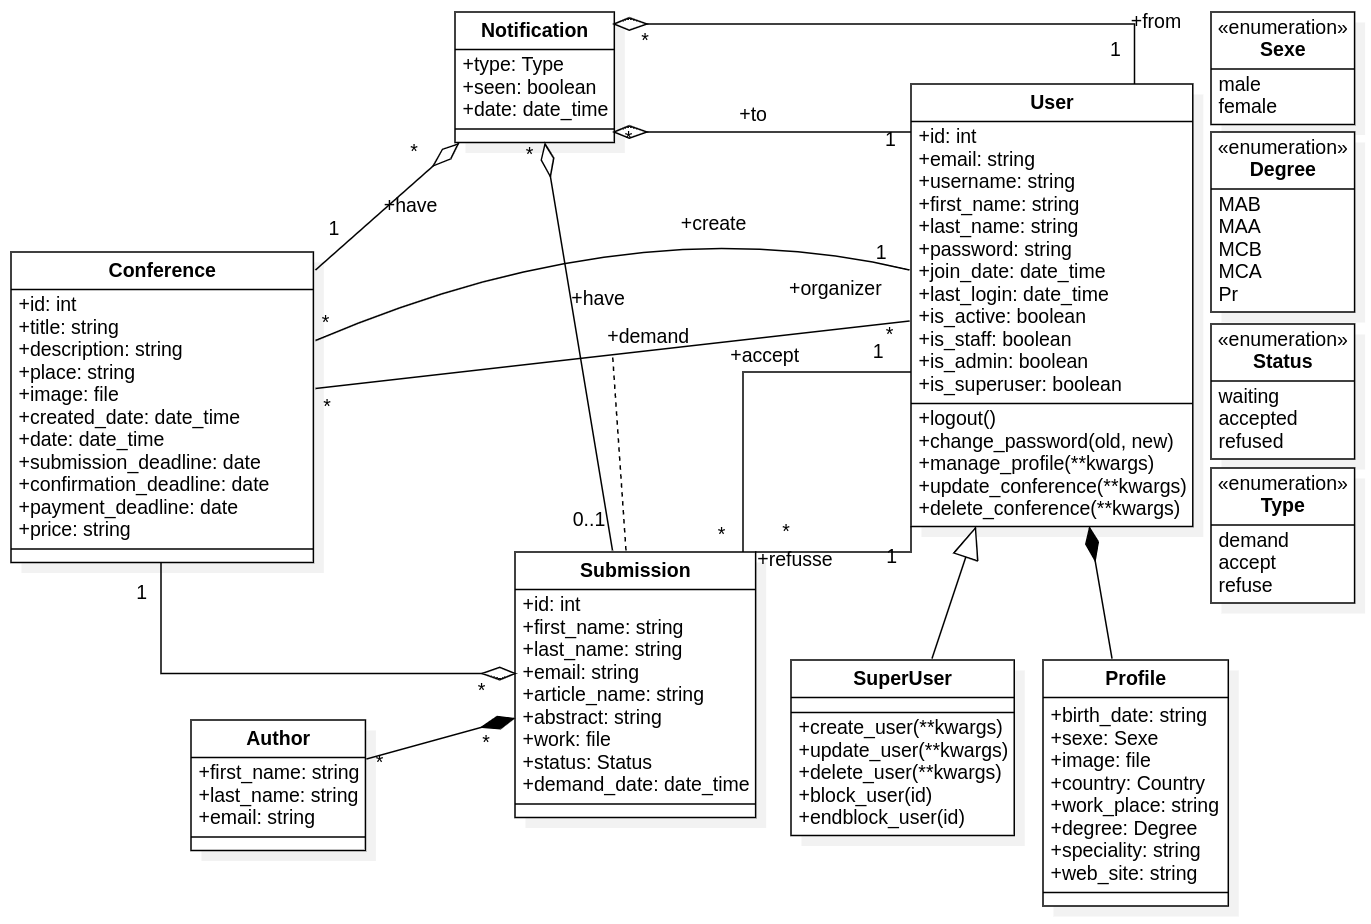
\includegraphics[width=\textwidth]{diagrams/class.png}
			\caption{class diagram}
			\label{fig:class-d}
		\end{figure}
	
	\subsection{Use case Diagram}
	In Figure \ref{fig:use-case-d} we diagram to introduce what can every actor do in this project.
	
		\begin{figure}[b]
			\centering
			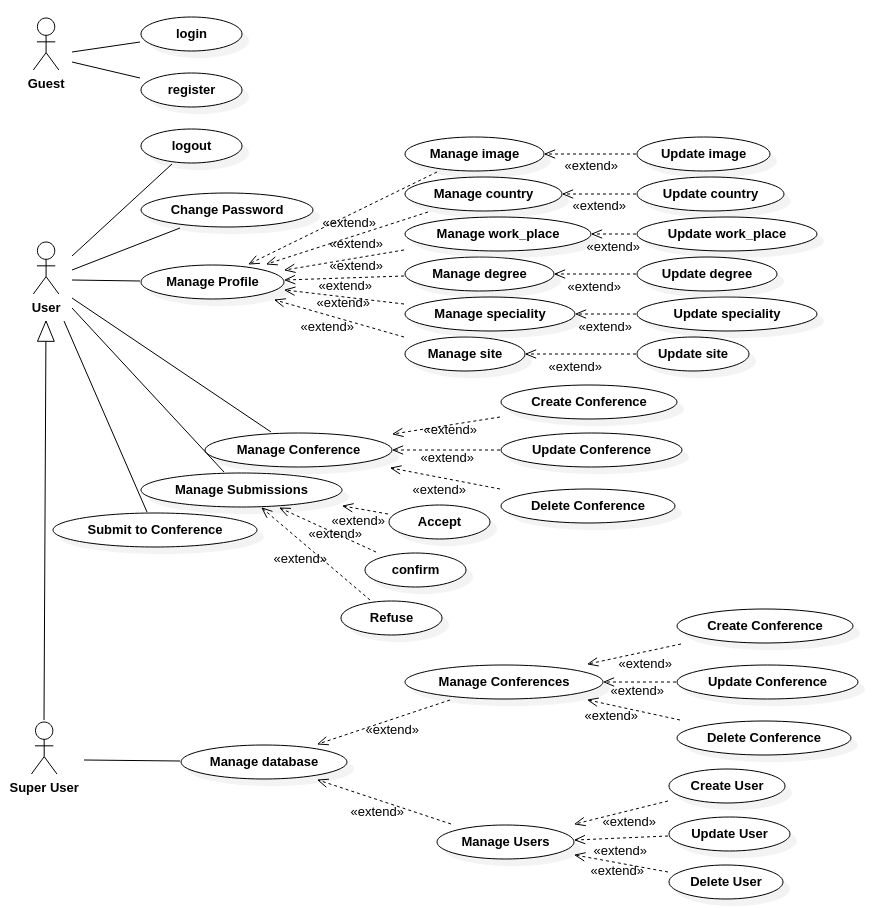
\includegraphics[width=\textwidth]{diagrams/use_case.png}
			\caption{use case diagram}
			\label{fig:use-case-d}
		\end{figure}
	
	\subsection{Sequence Diagrams}
	diagrams to figure out how each process is working behind the scene.
	
	
	\subsubsection{For login}
	In Figure \ref{fig:login-s-d} we have how the user can login
	
		\begin{figure}[b]
			\centering
			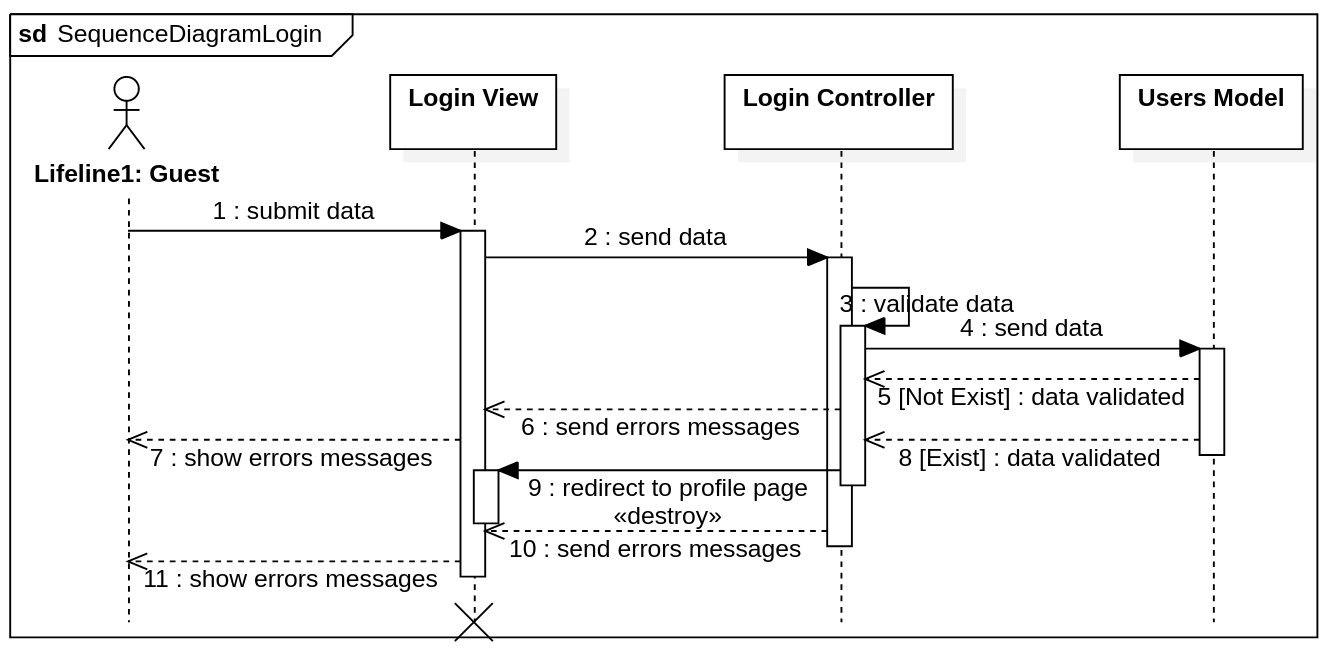
\includegraphics[width=\textwidth]{diagrams/login_sequence.png}
			\caption{login sequence diagram}
			\label{fig:login-s-d}
		\end{figure}
	
	\subsubsection{For register}
	In Figure \ref{fig:register-s-d} we have how to register as a new user
	
		\begin{figure}[b]
			\centering
			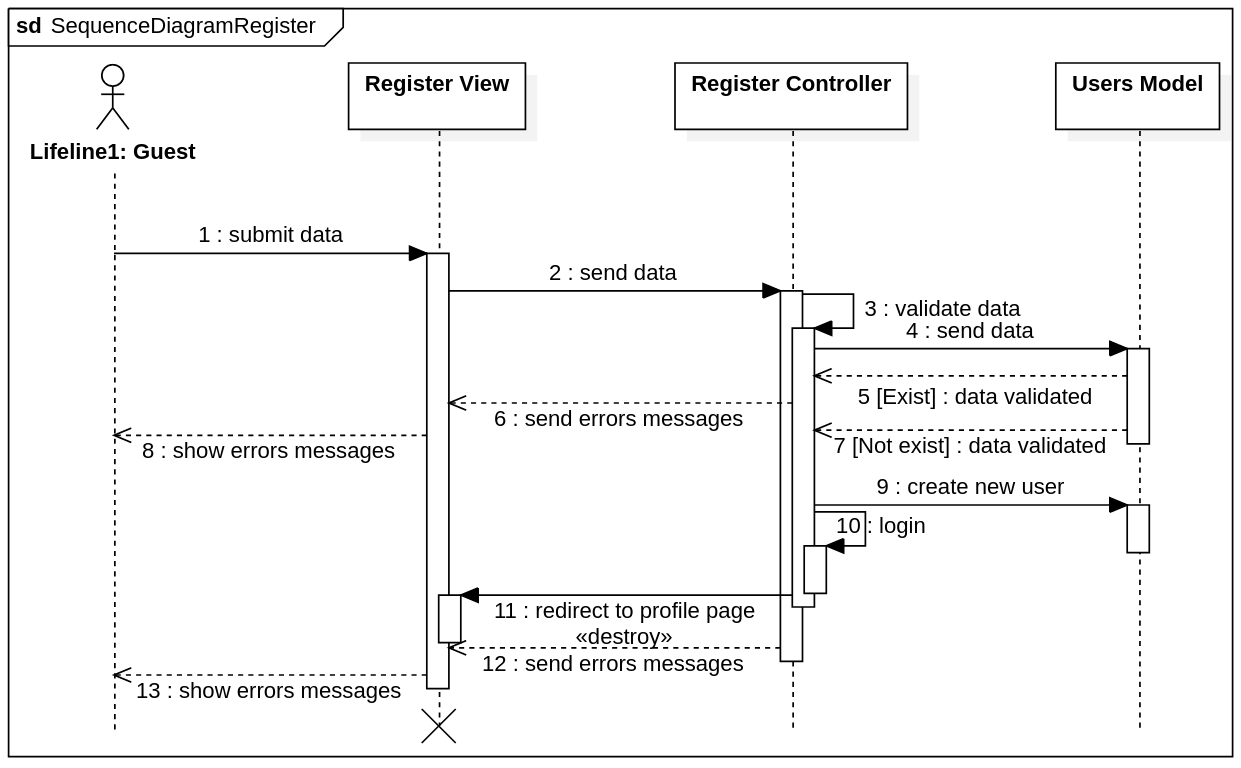
\includegraphics[width=\textwidth]{diagrams/register_sequence.png}
			\caption{register sequence diagram}
			\label{fig:register-s-d}
		\end{figure}
	
	\subsubsection{For create user}
	In Figure \ref{fig:user-create-s-d} we have how to create new user
	
		\begin{figure}[b]
			\centering
			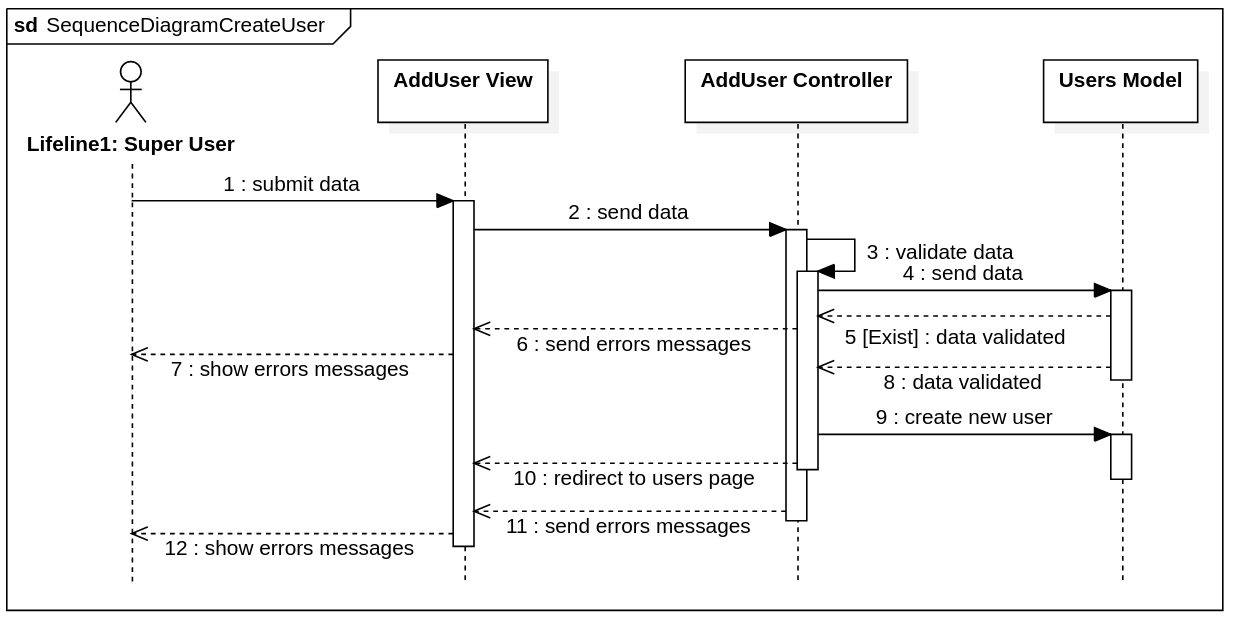
\includegraphics[width=\textwidth]{diagrams/user_create_sequence.png}
			\caption{create user sequence diagram}
			\label{fig:user-create-s-d}
		\end{figure}
	
	\subsubsection{For update user}
	In Figure \ref{fig:user-update-s-d} we have how to update user information
	
		\begin{figure}[b]
			\centering
			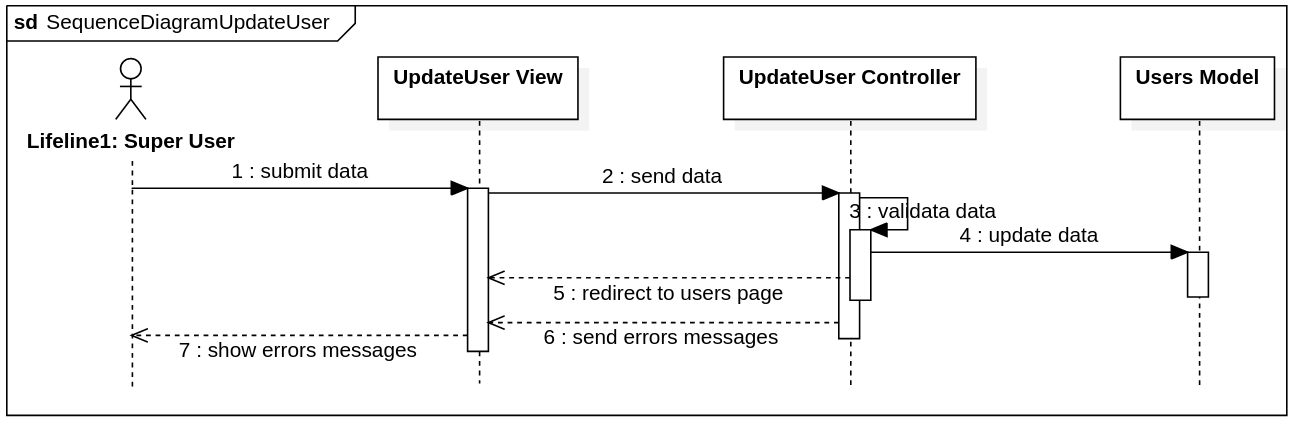
\includegraphics[width=\textwidth]{diagrams/user_update_sequence.png}
			\caption{update user sequence diagram}
			\label{fig:user-update-s-d}
		\end{figure}
	
	\subsubsection{For delete user}
	In Figure \ref{fig:user-delete-s-d} we have how to delete a user from the data base

		\begin{figure}[b]
			\centering
			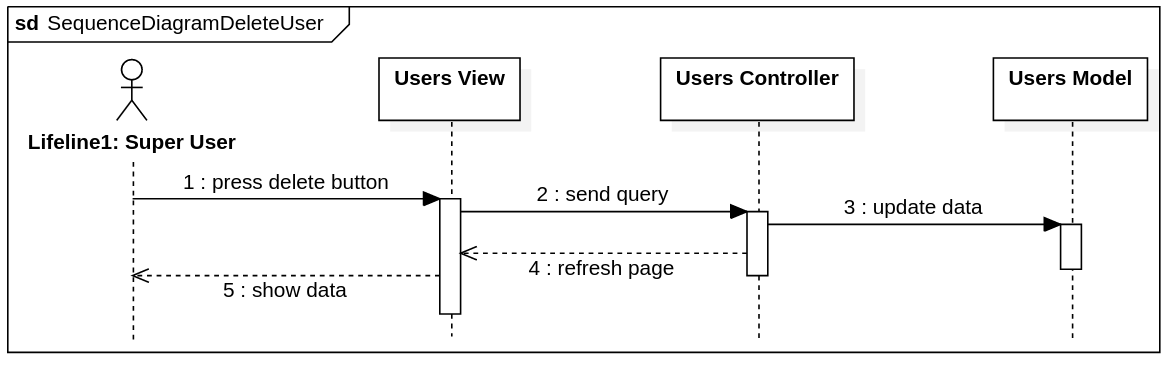
\includegraphics[width=\textwidth]{diagrams/user_delete_sequence.png}
			\caption{delete sequence diagram}
			\label{fig:user-delete-s-d}
		\end{figure}
	
	\subsubsection{For create conference}
	In Figure \ref{fig:conference-create-s-d} we have how to create new user
	
		\begin{figure}[b]
			\centering
			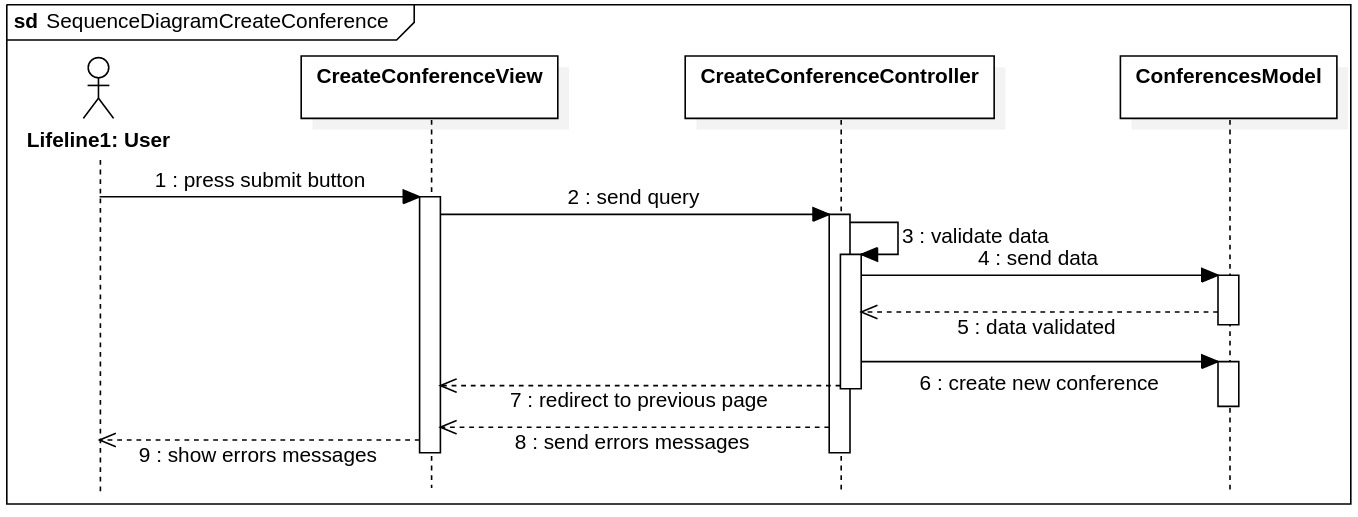
\includegraphics[width=\textwidth]{diagrams/conference_create_sequence.png}
			\caption{create user sequence diagram}
			\label{fig:conference-create-s-d}
		\end{figure}
	
	\subsubsection{For update conference}
	In Figure \ref{fig:conference-update-s-d} we have how to update user information
	
		\begin{figure}[b]
			\centering
			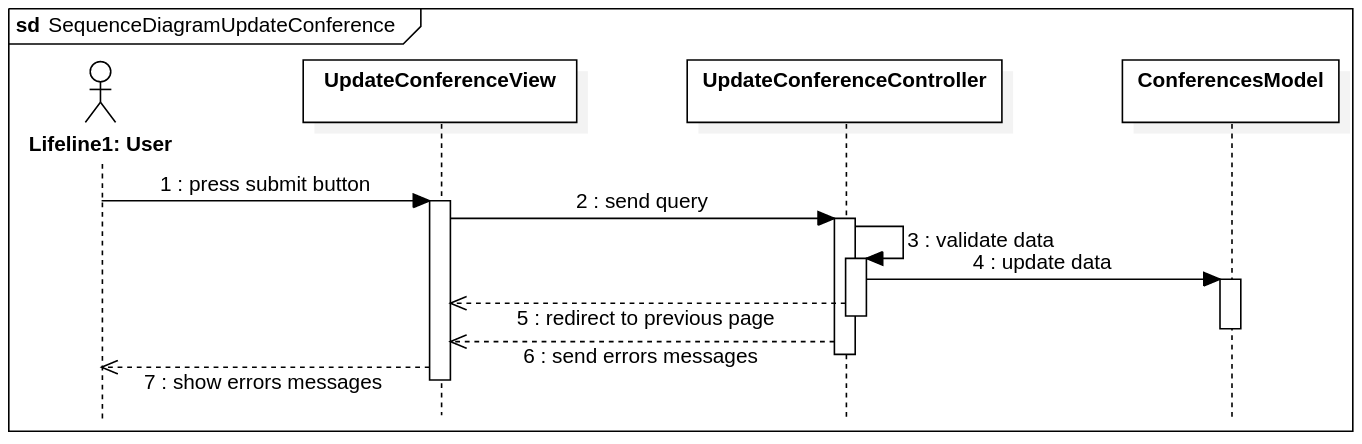
\includegraphics[width=\textwidth]{diagrams/conference_update_sequence.png}
			\caption{update user sequence diagram}
			\label{fig:conference-update-s-d}
		\end{figure}
	
	\subsubsection{For delete conference}
	In Figure \ref{fig:conference-delete-s-d} we have how to delete a user from the data base
	
		\begin{figure}[b]
			\centering
			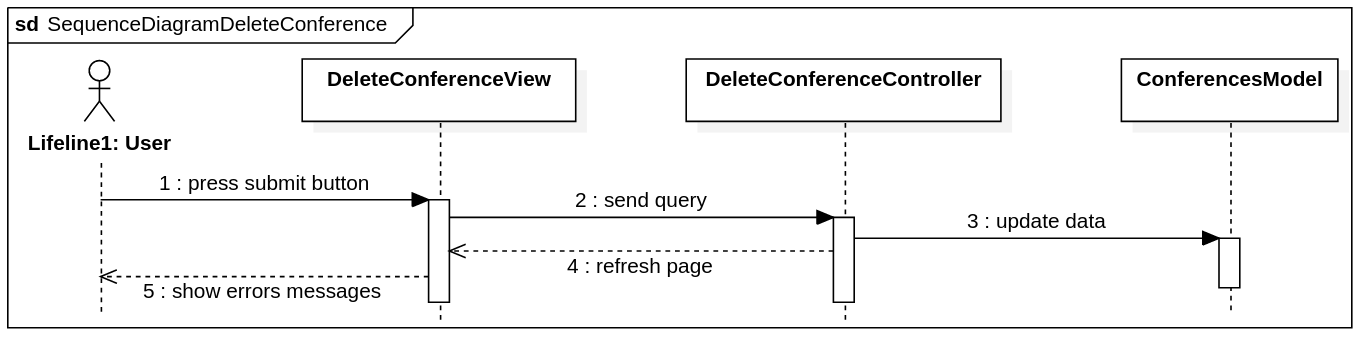
\includegraphics[width=\textwidth]{diagrams/conference_delete_sequence.png}
			\caption{delete sequence diagram}
			\label{fig:conference-delete-s-d}
		\end{figure}
	
	\subsubsection{For create submission}
	In Figure \ref{fig:submission-create-s-d} we have how to create new user
	
		\begin{figure}[b]
			\centering
			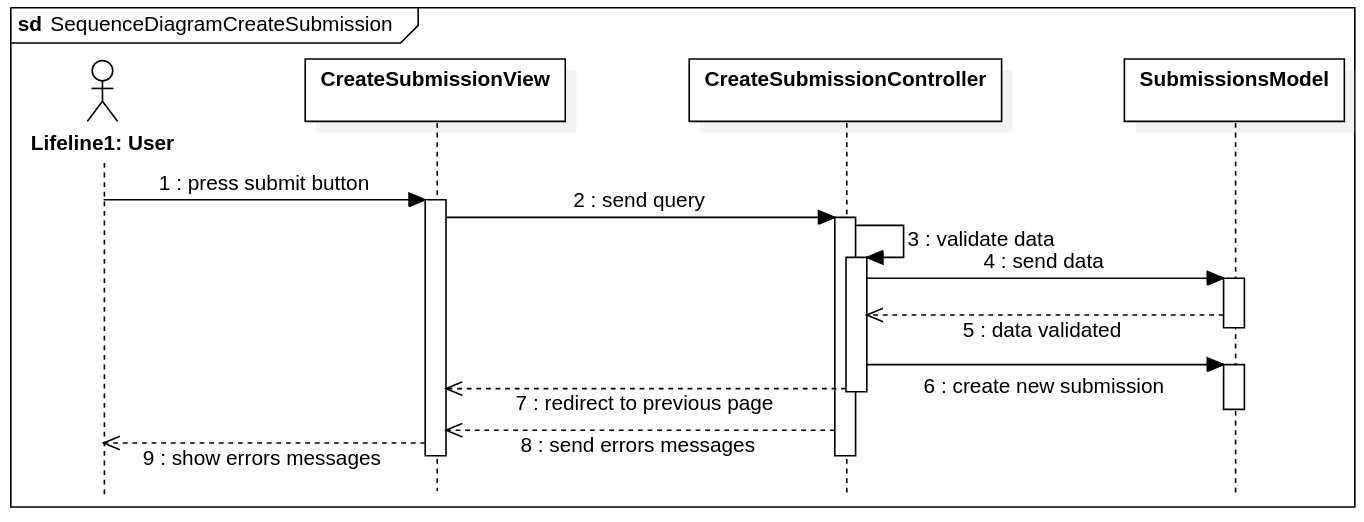
\includegraphics[width=\textwidth]{diagrams/submission_create_sequence.png}
			\caption{create user sequence diagram}
			\label{fig:submission-create-s-d}
		\end{figure}
	
	\subsubsection{For update submission}
	In Figure \ref{fig:submission-update-s-d} we have how to update user information
	
		\begin{figure}[b]
			\centering
			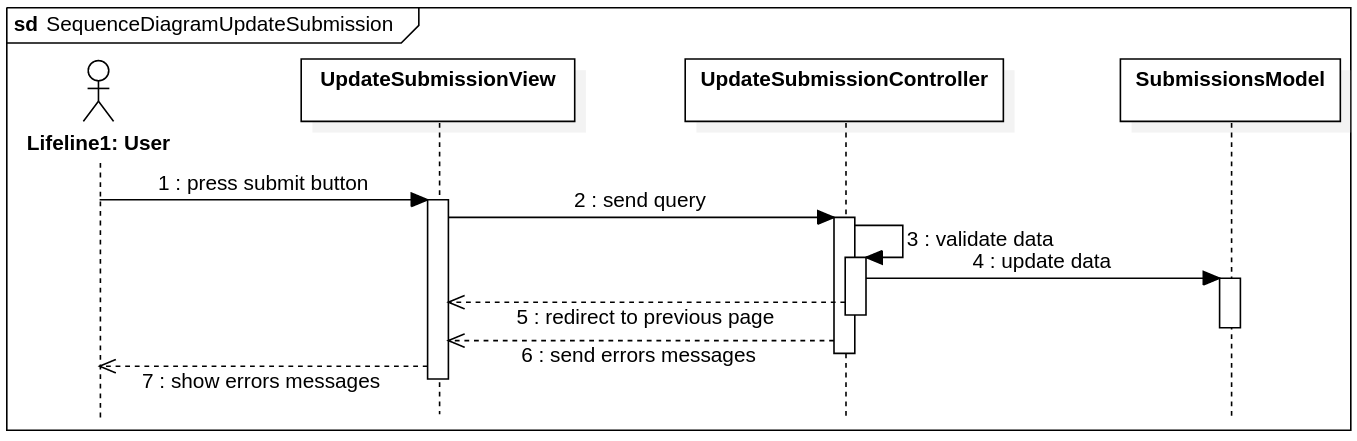
\includegraphics[width=\textwidth]{diagrams/submission_update_sequence.png}
			\caption{update user sequence diagram}
			\label{fig:submission-update-s-d}
		\end{figure}
	
	\subsubsection{For delete submission}
	In Figure \ref{fig:submission-delete-s-d} we have how to delete a user from the data base
	
		\begin{figure}[b]
			\centering
			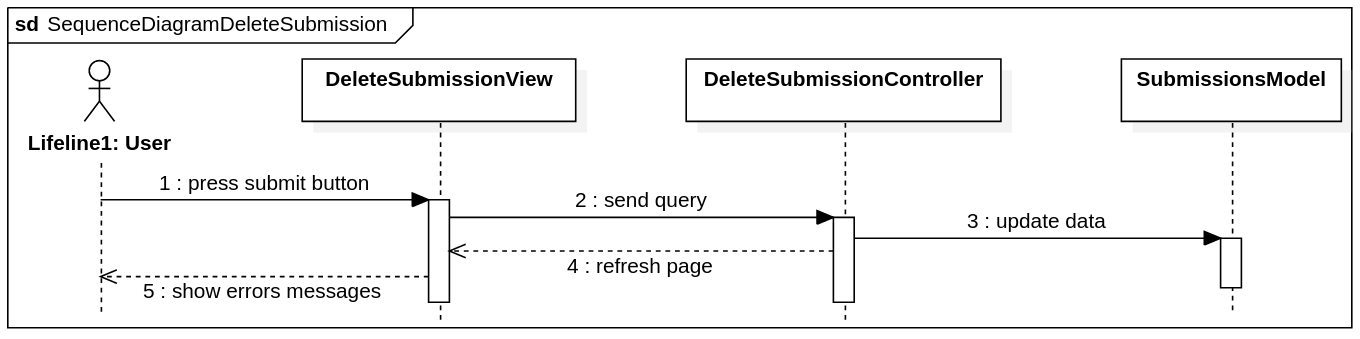
\includegraphics[width=\textwidth]{diagrams/submission_delete_sequence.png}
			\caption{delete sequence diagram}
			\label{fig:submission-delete-s-d}
		\end{figure}